\section{Analyse der Ausgangslage}

Dieses Kapitel untersucht die konkrete Ausgangssituation, in der das Projekt verankert ist.  
Basierend auf einem Workshop am Swiss Center for Design and Health (SCDH) sowie der übergeordneten Zielsetzung werden zentrale Probleme und Anforderungen identifiziert, die für die Entwicklung der geplanten Softwarelösung relevant sind.  
Die im vorangegangenen Kapitel~\ref{sec:Hintergrund und verwandte Arbeiten} dargestellten technischen Grundlagen und bestehenden Systeme bilden dabei die Grundlage für die folgende Analyse.

Zunächst wird der beobachtete Workshopverlauf beschrieben, um die praktische Anwendungssituation besser zu verstehen. Anschliessend werden daraus konkrete Anforderungen abgeleitet, welche die technische und gestalterische Umsetzung im weiteren Projektverlauf mitprägen.


\subsection{Beobachtungen im Workshop}
\label{sec:workshop}

Im Rahmen des Projekts wurde ein Workshop des SCDH besucht, der am 3.~April~2025 in Nidau stattfand. Auftraggeber des Workshops war das Wohnheim Humanitas aus Horgen. Ziel war es, die geplanten Arbeitsabläufe im zukünftigen Neubau des Wohnheims im Zusammenhang mit einem Assistenzkran realitätsnah zu simulieren und zu evaluieren.

\begin{figure}[H]
  \centering
  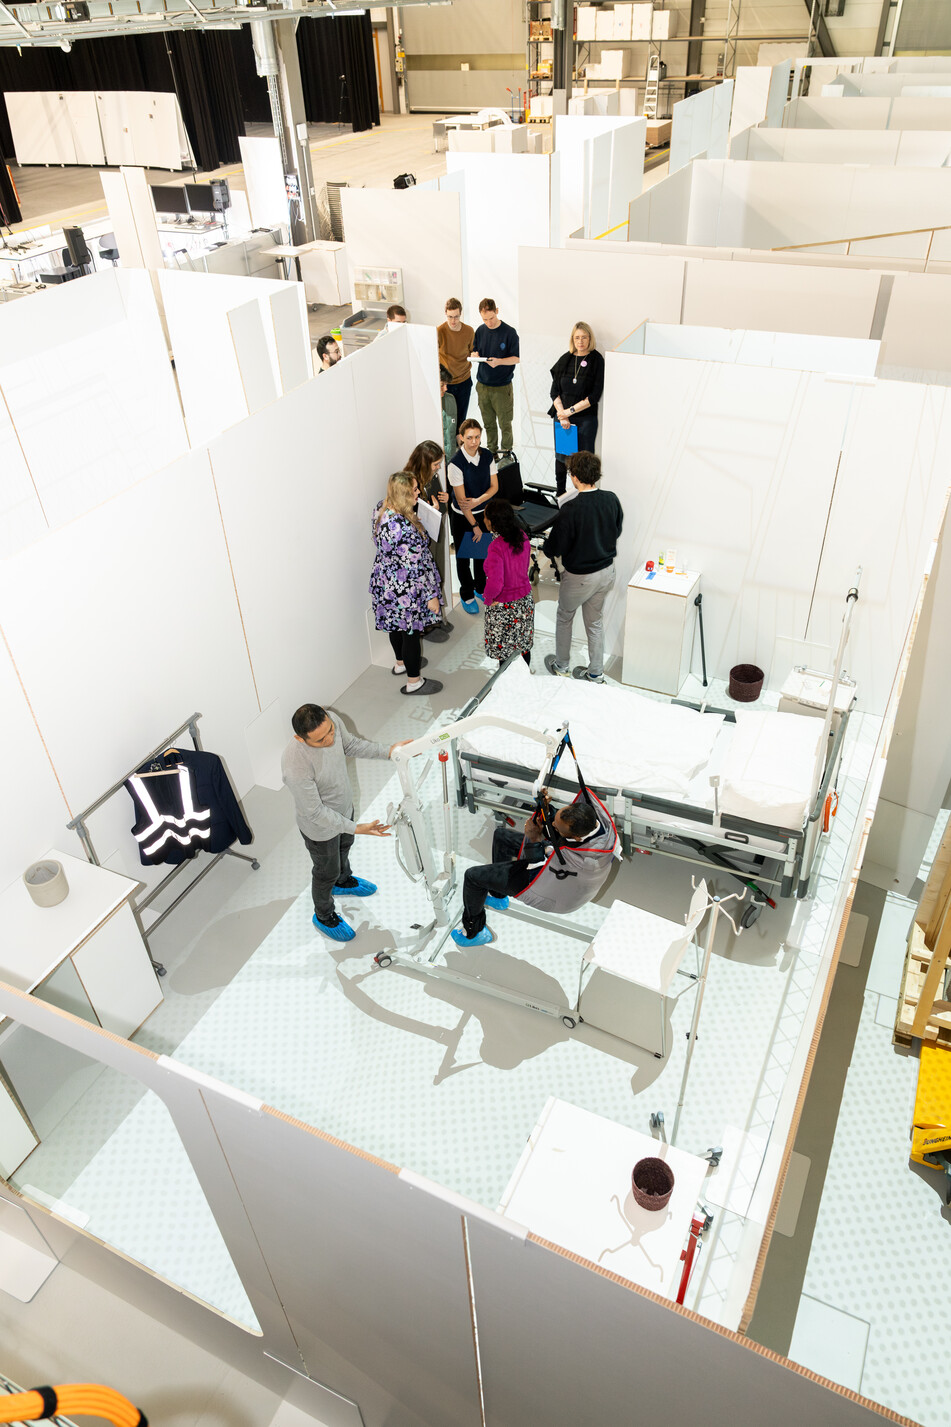
\includegraphics[width=0.5\linewidth]{graphics/workshop.jpg}
  \caption{Simulation der Barrierefreiheit im Neubau der Humanitas Stiftung}
  \cite{scdh_humanitas_image_nodate}
  \label{fig:humanitas_image}
\end{figure}
\clearpage


Hierzu wurden die bestehenden Baupläne auf die 1:1-Projektionsfläche überspielt. Das Workshopteam nutzte diese Fläche, um verschiedene alltägliche Situationen direkt vor Ort nachzustellen und auszuführen. Die Teilnehmenden konnten sich so durch Rollenspiel ein Bild von typischen Interaktionen und Bewegungsabläufen im geplanten Raumkonzept machen.

Der Ablauf des Workshops war in drei Phasen gegliedert:

\begin{itemize}
  \item \textbf{Briefing:} Gemeinsame Einführung in die Zielsetzung und den Planungsstand.
  \item \textbf{Simulation:} Aktives Begehen und Durchspielen der Szenarien auf der Projektionsfläche.
  \item \textbf{Debriefing:} Diskussion und Reflexion von Verbesserungsmöglichkeiten am Raumkonzept.
\end{itemize}

Besonderes Augenmerk lag auf den Phasen \textit{Briefing} und \textit{Debriefing}, da diese für das Projekt relevant sind: In diesen Momenten hätten digitale Zeichen- und Interaktionsmöglichkeiten den Austausch zwischen Teilnehmenden nachweislich unterstützen können (siehe auch Abschnitt~\ref{sec:verbesserungspotentiale}).



\subsection{Abgeleitete Anforderungen aus dem Workshop}

Die Beobachtungen vor Ort bestätigten nicht nur die Anforderungen aus der ursprünglichen Aufgabenstellung, sondern lieferten zusätzliche Einblicke in praktische Herausforderungen.

Folgende zusätzliche Anforderungen und Erkenntnisse wurden im Workshop identifiziert:

\begin{itemize}
  \item \textbf{Niederschwellige Bedienung:} Die Lösung muss auch von Personen ohne technische Vorkenntnisse oder mit sprachlichen Barrieren genutzt werden können.
  \item \textbf{Echtzeit-Funktionalität:} Änderungen müssen sofort sichtbar sein, um den Diskussionsfluss nicht zu unterbrechen.
  \item \textbf{Zugängliche Bedienung vom Platz aus:} Teilnehmende sollen Zeichnungen oder Korrekturen vornehmen können, ohne sich zur Projektionsfläche bewegen zu müssen.
  \item \textbf{Unterstützung spontaner Visualisierung:} Ideen und Probleme (z.\,B. Türrichtung, Gerätepositionierung) müssen spontan eingezeichnet werden können, um Missverständnisse zu vermeiden.
\end{itemize}

Diese Anforderungen belegen, dass ein interaktives Zeichensystem einen echten Mehrwert für solche Workshops darstellen kann, nicht nur zur Planung, sondern auch zur Verbesserung von Kommunikation, Teilhabe und gemeinsamen Entscheidungen.

